\customsection{Introducción}
\subsection{Contexto introductorio}
No es para nadie una sorpresa que durante este siglo, las nuevas generaciones que nacen rodeadas de la tecnología y están cambiando las costumbres y el paradigma actual de lo que significa una vivienda, con una sociedad cada vez más relacionada con la tecnología, nuevos desafíos de diseño e implementación se plantean para satisfacer las expectativas de las nuevas generaciones.
\vspace{0.5cm}\\
Básicamente el más importante beneficio utilizar la tecnología en viviendas comerciales es el proveer de servicios y facilidades a personas discapacitadas y ancianos \cite{GiralSala2016}, por otra parte, tenemos beneficios de monitorización y la capacidad de añadir herramientas que permitan la integración con redes eléctricas inteligentes. La popularidad de sistemas inteligentes ha venido incrementando debido al confort adicional, y herramientas de seguridad que pueden recibir los usuarios. 
\vspace{0.5cm}\\
Por lo tanto, hay ciertos factores que deben ser tenidos en cuenta a la hora de diseñar un sistema de control y monitoreo de la vivienda, en este documento se explicará el proceso de diseño e implementación de un software para el manejo inteligente de una vivienda del Solar Decathlon Latinoamérica utilizando diferentes tecnologías de \textit{frontend} y \textit{backend}
\vspace{0.5cm}\\
La arquitectura desarrollada se puede describir en 3 productos:
 
\begin{enumerate}
	\item Un servicio de \textit{backend} serverless basado en: un broker de Mqtt, un servicio de almacenamiento de datos tipo S3, una base de datos relacional tipo MySql e interfaces http basadas en funciones de nube. 
	\item Un programa encargado de administrar y controlar todas las rutinas de comunicación, reporte y almacenamiento en el sitio de control con su respectiva interfaz de usuario.
	\item Una aplicación celular capaz de monitorear y controlar los datos generados localmente y los actuadores de la vivienda del Solar Decathlon.
\end{enumerate}


%\subsection{Planteamiento del problema}

Hoy en día las tecnologías orientadas internet y la mayoría de los objetos utilizados en la cotidianidad, en general, están cada vez más relacionadas entre sí; el pasado año se vio un incremento de 2.79 billones de nuevos dispositivos conectados a la red de redes (entre los cuales no solo se encuentran celulares computadores y tablets). Nuevos dispositivos como aires acondicionados, televisores y electrodomésticos en general son lanzados al mercado con la capacidad de comunicarse con el usuario a través de aplicaciones web o dispositivos móviles día tras día. Lo anterior se debe al aumento en los desarrollos de hardware y software para sistemas con la capacidad de acceso a la red; es decir, con la capacidad de acceder a comunicaciones inalámbricas, servidores locales, servicios en la nube, entre otras propuestas.
\vspace{0.5cm}\\
Teniendo en cuenta lo anterior, muchos sistemas basados en diseños embebidos y/o tarjetas de desarrollo CPU se han propuesto como forma de integración y aplicación de sistemas de domótica en el hogar. La mayoría de estos proyectos o aplicativos son pensados para automatizar tareas específicas o agregarle una componente de comunicación remota al hogar. Si bien estos son puntos atractivos para un consumidor, el concepto de vivienda inteligente se puede expandir por más terrenos, tan diversos como el que se presentará en este documento.
\vspace{0.5cm}\\
Un concepto tan abierto y ventajoso como el de la vivienda inteligente o el internet de las cosas puede ser utilizado en el marco del concurso Solar Decatlón Latín América, el cual plantea el desarrollo de un proyecto de vivienda residencial amigable con el medio ambiente, donde el diseño arquitectónico ganador se decide en base a 10 indicadores cada uno con 100 puntos calificados de manera cualitativa y cuantitativa por los jueces.
\vspace{0.5cm}\\
Para la porción de la puntuación que es calificada de manera cuantitativa los jueces utilizan medidores que, dependiendo del indicador, puede corresponder para monitorear o medir el consumo eléctrico, temperatura, humedad, picos de consumo (3 kilo watts) donde se establece un valor de mínimo y máximo para un rango de puntos desde cero hasta la máxima calificación.
\vspace{0.5cm}\\
Considerando lo anterior, se plantea realizar la mejor aproximación tecnológica para cumplir de manera más acercada los indicadores de: eficiencia energética, innovación, balance eléctrico energético y condiciones de confort, puesto que son aquellos que pueden ser solucionados gestionados y monitoreados por tecnologías actuales. Basándose en lo expuesto anteriormente se plantea la siguiente pregunta al problema de ingeniería:
\vspace{0.5cm}\\
¿Cómo diseñar e implementar un sistema software que permita la gestión de cargas eléctricas y el monitoreo de variables físicas de manera local y remota para el concurso del Solar Decatlón latín América?.
%\subsection{Justificación}
Respecto a la vivienda inteligente o la domótica en el hogar, se puede decir que la literatura es amplia y que existen diferentes propuestas comerciales de desarrollo como lo son: Calaos, Domoticz, Home Assistant, OpenHAB, OpenMotics, donde cada marca propone su marco de trabajo, y diferentes plataformas de desarrollo tanto software como hardware. Una desventaja de estas propuestas es su interfaz hardware, en la mayoría de los casos el hardware adicional corresponde a dispositivos desarrollados y mantenidos por ellos mismos, lo que significa que limita la escalabilidad de las
\vspace{0.5cm}\\
Las anteriores tecnologías son propuestas donde un centro de mando controla dispositivos externos, pero, por otra parte, si pensamos en cada módulo hardware con la capacidad de conectarse a la red de redes de manera independiente (Iot) como lo hace la propuesta realizada el en proyecto del “Smart switch” \cite{GiralSala2016}; se tiene como ventaja la independencia sobre las características físicas del hogar o de la capacitación técnica del instalador del sistema, pero como desventaja, al momento de escalar el problema a un mayor número de circuitos se pueden presentar problemas de saturación de la red inalámbrica (wifi) y sería más costoso debido al hardware adicional para cada nuevo circuito que se desee controlar.
\vspace{0.5cm}\\
Teniendo en cuenta las comparaciones anteriores, se podría pensar que un sistema que englobe varios sub sistemas podría ser el adecuado desde el punto de vista de la escalabilidad, pero esa no es la única razón; Hoy en día los métodos de generación alternativa y energía renovable se encuentran en crecimiento, por lo que nace la necesidad de interconectar redes eléctricas inteligentes, es decir, una red con un componente de generación y consumo tanto como AC y DC. Este tipo de topología eléctrica se le conoce como nanogrid, y se ampliará la teoría respecto a este concepto en futuras secciones del documento. Esta topología eléctrica añade como variable la generación eléctrica junto con una nueva forma fisica de energía (corriente directa).
\vspace{0.5cm}\\
Inclusive, se puede observar que artículos académicos se han dedicado a analizar este concepto en el contexto Colombiano,  por ejemplo un estudio sobre microgrids mencionó la importancia y necesidad de implementar viviendas inteligentes como se ve a continuación: “desde el contexto de seguridad eléctrica, equidad social y mitigación del impacto ambiental en Colombia, el sistema energético debe afrontar los nuevos retos requeridos para satisfacer la demanda. Desde un punto de vista técnico, es necesario dotar la red tradicional con las características de una red inteligente ”. 
\vspace{0.5cm}\\
Pero ¿acaso una red inteligente implica una casa inteligente? La respuesta es; parcialmente sí. Considerando que hoy en día toda vivienda realiza un monitoreo o medición de al menos 2 variables críticas; el consumo eléctrico, y el consumo de agua, ambos son de interés para la compañía prestadora de servicios públicos en la vivienda.
\vspace{0.5cm}\\
Resaltando la importancia de las anteriores variables físicas y teniendo en cuenta el modelo de nanogrid al cual podría llegar a ser una vivienda; la gestion de informacion adicional a la necesaria para cumplir la domótica resalta al a vista. En adición, estos componentes de generación y consumo eléctrico son la base para hablar sobre el impacto ambiental de las costumbres internas de los habitantes de un hogar, que resulta de vital interés para la optimización de los 4 ítems de calificación en el solar decathlon.
\vspace{0.5cm}\\
Finalizando, una propuesta integral de domótica y gestión inteligente de información como la que se presenta en este documento facilita la verificación y el cumplimiento de los ítems anteriormente mencionados, contemplando que el sistema quedara diseñado de tal manera que sea fácil la escalabilidad para aspectos como; seguridad, aseguramiento contra accidentes (incendio), viviendas de diferente tamaño, interfaz de voz y video.


%\subsection{Objetivos}

\subsubsection{Objetivo general}
Implementar un sistema software para una vivienda del Solar Decathlon capaz de gestionar el control y la medición de variables físicas de manera local y remota.
\subsubsection{Objetivos especificos}
\begin{itemize}
	\item Diseñar una API que permita implementar interfaces gráficas, haciendo uso de imágenes personalizadas, para lograr una interacción amigable con el usuario.
	\item Implementar una aplicación software que funcione en el sitio y le permita al usuario gestionar la información de interés y controlar las cargas eléctricas.
	\item Implementar un aplicativo móvil que le permita al usuario tener la experiencia de interactuar con una vivienda inteligente.
\end{itemize}


\subsection{Lineamientos de desarrollo}
Debido a la naturaleza del proyecto, parte de los aspectos definidos al momento de establecer el anteproyecto fueron unas necesidades funcionales explicadas en el formato \ref{tab0}.

% Please add the following required packages to your document preamble:
% \usepackage[table,xcdraw]{xcolor}
% If you use beamer only pass "xcolor=table" option, i.e. \documentclass[xcolor=table]{beamer}

\begin{longtable}[c]{lllc}
\hline
\multicolumn{1}{|l|}{
\begin{tabular}[c]{@{}l@{}}
	
\includegraphics[width=1cm]{figuras/uv_logo.png}
\end{tabular}
} 
& 
\multicolumn{2}{l|}{\cellcolor[HTML]{808080}{\color[HTML]{FFFFFF} \textbf{
\begin{tabular}[c]{@{}l@{}}Universidad del Valle\\--Implementación de un gestionado de recursos\\ para el hogar con inteligencia ambiental. ---\end{tabular}}}}
&
\multicolumn{1}{c|}{\textbf{\begin{tabular}[c]{@{}c@{}}Rev:\\ 003\end{tabular}}} \\ \hline
\endfirsthead
%
\endhead
%
\multicolumn{2}{|l|}{\textbf{\begin{tabular}[c]{@{}l@{}}Título:\\   ESPECIFICACIÓN DE \\ REQUERIMIENTOS \\ FUNCIONALES\end{tabular}}} & \multicolumn{1}{l|}{\textbf{\begin{tabular}[c]{@{}l@{}}Documento :\\ ERF-000\end{tabular}}} & \multicolumn{1}{c|}{\textbf{\begin{tabular}[c]{@{}c@{}}Página :\\ 1 de 1\end{tabular}}} \\ \hline
 &  &  & \multicolumn{1}{l}{} \\ \hline
\rowcolor[HTML]{808080} 
\multicolumn{4}{|c|}{\cellcolor[HTML]{808080}\textbf{REVISIÓN HISTÓRICA}} \\ \hline
\rowcolor[HTML]{808080} 
\multicolumn{1}{|l|}{\cellcolor[HTML]{808080}\textbf{Rev.}} & \multicolumn{1}{l|}{\cellcolor[HTML]{808080}\textbf{Descripción del Cambio}} & \multicolumn{1}{l|}{\cellcolor[HTML]{808080}\textbf{Autor}} & \multicolumn{1}{l|}{\cellcolor[HTML]{808080}\textbf{Fecha}} \\ \hline
\multicolumn{1}{|l|}{001} & \multicolumn{1}{l|}{Construcción del documento} & \multicolumn{1}{l|}{\begin{tabular}[c]{@{}l@{}}Juan David Ramirez\\ Villegas\end{tabular}} & \multicolumn{1}{l|}{18/03/2017} \\ \hline
\multicolumn{1}{|l|}{002} & \multicolumn{1}{l|}{Correcciones} & \multicolumn{1}{l|}{\begin{tabular}[c]{@{}l@{}}Juan David Ramírez\\ Villegas\end{tabular}} & \multicolumn{1}{l|}{15/11/2017} \\ \hline
\multicolumn{1}{|l|}{003} & \multicolumn{1}{l|}{Revisión} & \multicolumn{1}{l|}{\begin{tabular}[c]{@{}l@{}}Juan David Ramírez\\ Villegas\end{tabular}} & \multicolumn{1}{l|}{18/12/2017} \\ \hline
 &  &  & \multicolumn{1}{l}{} \\ \hline
\rowcolor[HTML]{808080} 
\multicolumn{1}{|l|}{\cellcolor[HTML]{808080}\textbf{Ref \#}} & \multicolumn{2}{l|}{\cellcolor[HTML]{808080}\textbf{Funciones}} & \multicolumn{1}{l|}{\cellcolor[HTML]{808080}\textbf{Categoría}} \\ \hline
\multicolumn{1}{|l|}{1.0} & \multicolumn{2}{l|}{USER APP (application móvil)} & \multicolumn{1}{c|}{\textbf{O}} \\ \hline
\multicolumn{1}{|l|}{1.1} & \multicolumn{2}{l|}{\begin{tabular}[c]{@{}l@{}}El usuario debe poder acceder a la \\ información medida en tiempo real.\end{tabular}} & \multicolumn{1}{c|}{\textbf{E}} \\ \hline
\multicolumn{1}{|l|}{1.2} & \multicolumn{2}{l|}{\begin{tabular}[c]{@{}l@{}}El usuario debe poder acceder a los datos \\ históricos recopilados en el mes y la \\ relación de sus gastos con ellos.\end{tabular}} & \multicolumn{1}{c|}{\textbf{O}} \\ \hline
\multicolumn{1}{|l|}{1.3} & \multicolumn{2}{l|}{\begin{tabular}[c]{@{}l@{}}El usuario debe poder cambiar los \\ parámetros de configuración escogidos\\  por defecto para la vivienda del\\  Solar Decathlon.\end{tabular}} & \multicolumn{1}{c|}{\textbf{E}} \\ \hline
\multicolumn{1}{|l|}{1.4} & \multicolumn{2}{l|}{\begin{tabular}[c]{@{}l@{}}El usuario debe recibir recomendaciones\\  para mejorar su entorno y su huella \\ hídrica cada cierto tiempo.\end{tabular}} & \multicolumn{1}{c|}{\textbf{E}} \\ \hline
\multicolumn{1}{|l|}{1.5} & \multicolumn{2}{l|}{\begin{tabular}[c]{@{}l@{}}La aplicación notificará al usuario\\ cuando la factura de energía o agua\\  esté vencida.\end{tabular}} & \multicolumn{1}{c|}{\textbf{O}} \\ \hline
\multicolumn{1}{|l|}{1.6} & \multicolumn{2}{l|}{\begin{tabular}[c]{@{}l@{}}El usuario debe ser capaz de ver un \\ índice del impacto ambiental de su\\  estilo de vida basado en datos \\ cualitativos y cuantitativos\end{tabular}} & \multicolumn{1}{c|}{\textbf{E}} \\ \hline
\multicolumn{1}{|l|}{1.7} & \multicolumn{2}{l|}{\begin{tabular}[c]{@{}l@{}}El sistema debe ser capaz de notificar \\ las pérdidas eléctricas, y por consiguiente\\  económicas, de un mal uso de los horarios\\  establecidos por defecto.\end{tabular}} & \multicolumn{1}{c|}{\textbf{O}} \\ \hline
\multicolumn{1}{|l|}{2.0} & \multicolumn{2}{l|}{HOUSE MANAGER (Aplicación en sitio)} & \multicolumn{1}{c|}{\textbf{E}} \\ \hline
\multicolumn{1}{|l|}{2.1} & \multicolumn{2}{l|}{\begin{tabular}[c]{@{}l@{}}El sistema debe mostrar gráficamente \\ la cantidad de agua y potencia consumida\\  durante el día contrastándolas con un \\ valor máximo recomendado.\end{tabular}} & \multicolumn{1}{c|}{\textbf{E}} \\ \hline
\multicolumn{1}{|l|}{2.2} & \multicolumn{2}{l|}{\begin{tabular}[c]{@{}l@{}}Por defecto, el uso de las cargas \\ eléctricas más significativas debe\\  programarse durante los picos de \\ generación en la casa. Estos horarios \\ podrán ser modificados bajo una \\ advertencia de uso no eficiente.\end{tabular}} & \multicolumn{1}{c|}{\textbf{E}} \\ \hline
\multicolumn{1}{|l|}{2.3} & \multicolumn{2}{l|}{\begin{tabular}[c]{@{}l@{}}El usuario debe poder acceder \\ a la información medida en tiempo real.\end{tabular}} & \multicolumn{1}{c|}{\textbf{E}} \\ \hline
\multicolumn{1}{|l|}{2.4} & \multicolumn{2}{l|}{\begin{tabular}[c]{@{}l@{}}El sistema debe poder comunicarse \\ con una base de datos que represente \\ todas las variables y el estado de los \\ circuitos de la vivienda.\end{tabular}} & \multicolumn{1}{c|}{\textbf{E}} \\ \hline
\caption{Requerimientos Funcionales del sistema}
\label{tab0}\\
\end{longtable}
La columna de la categoría indica si el requerimiento indicado es uno esencial (E) u opcional (O) para el desarrollo del sistema. Este documento será de gran importancia puesto que definió los lineamientos de desarrollo de todas las aplicaciones.




\subsection{Diseño Generalizado}

El sistema se diseñó con las mejores condiciones de: modularidad, costo, tamaño y escalabilidad. Para cada uno de estas características se escogieron tecnologías y se desarrollaron funciones claves. 
\vspace{0.5cm}\\
Desde la perspectiva de la modularidad, se desarrollaron aplicaciones de frontend capaces de integrarse con 2 tipos de protocolos de comunicación: Mqtts y Https; además, para acceder a los servicios de la nube se implementó el servicio de backend en la plataforma ``Google Cloud Plataform'' puesto que permite utilizar de la mejor manera todos los servicios de google: su asistente de voz, su interfaz de inteligencia artificial, sus servicios de autenticación, su red privada de fibra óptica (que es de las más rápidas y de mayor cobertura), entre otros.
\vspace{0.5cm}\\
En cuanto al costo, se utilizaron tecnologías de backend totalmente escalables tipo serverless para ajustar los gastos a únicamente los necesarios, teniendo en cuenta que las pruebas a gran escala estuvieron lejos del alcance de este proyecto, aún así se desarrolló toda la arquitectura pensando en la necesidad de optimizar en la mayor medida los gastos. Teniendo en cuenta que no se hicieron pruebas a gran escala los servicios de backend fueron posibles gracias a las cuotas gratuitas del mayorista utilizado para desplegar el servicio (Google).
\vspace{0.5cm}\\
En cuanto al requerimiento de escalabilidad, la decisión de diseñar serverless jugó el papel más importante: Los servicios servirles le permitieron a la aplicación ser diseñada para permanecer funcional sin hacer ningún cambio inclusive con 4000 usuarios (esta última apreciación es teórica puesto que no se hicieron pruebas a esa escala).
\vspace{0.5cm}\\
Para comprender mejor el producto, se puede observar en la figura \ref{diagramaGeneralizado} un diagrama generalizado de los componentes de software del sistema, donde principalmente los desarrollos hacen parte de 3 grandes bloques: el bloque de la nube, el bloque del dispositivo embebido (Raspberry), y el bloque del dispositivo móvil (Android).
\vspace{0.5cm}\\
\begin{figure}[htbp]
	\centering
	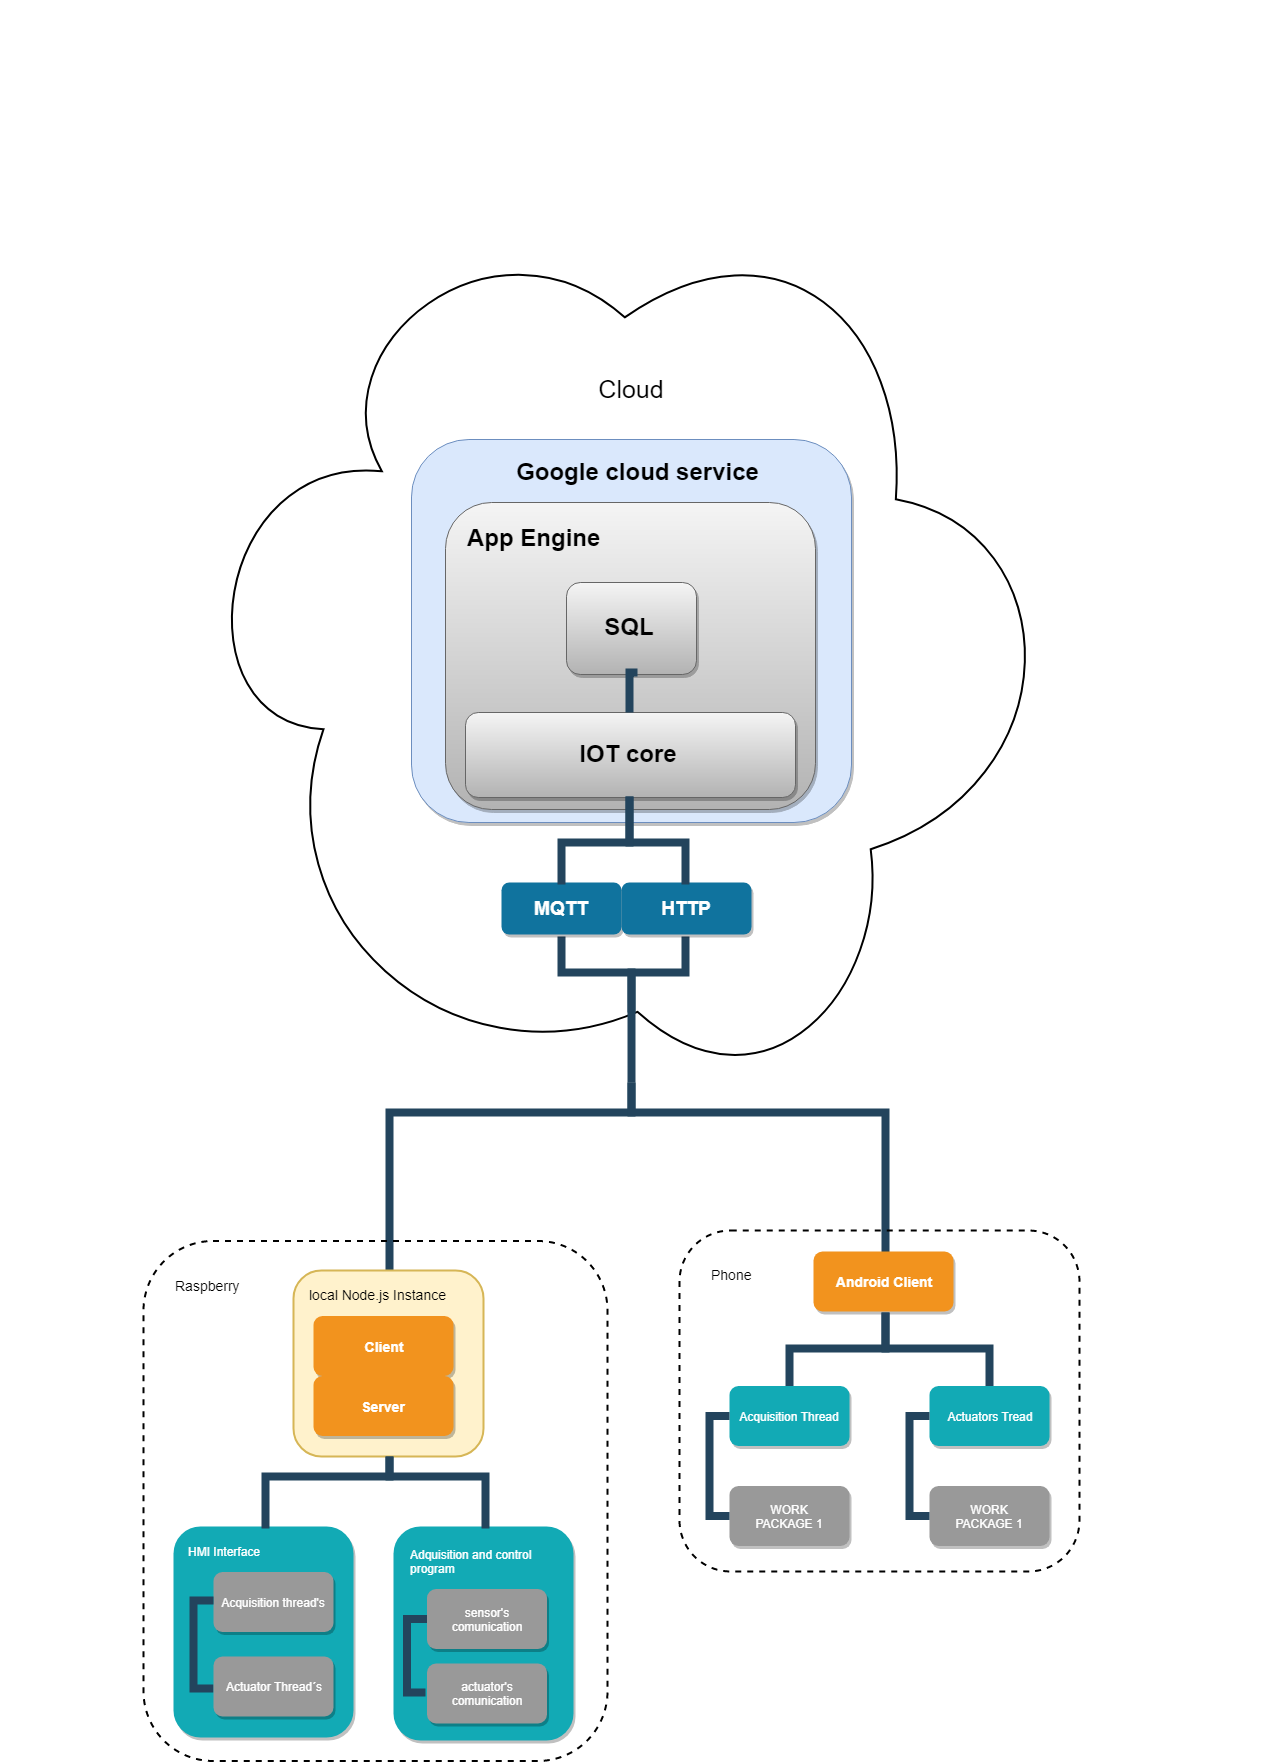
\includegraphics[width=10cm]{figuras/GeneralDiagram.png}
	\caption{Diagrama generalizado de las estructuras de software. Fuente: propia}	
	\label{diagramaGeneralizado}
\end{figure}

El producto del backend se implementó en el servicio de Google Cloud Services y utilizó los siguientes elementos para su funcionamiento: Un ``Storage version 3 system'' conectado a la red privada de Google para el almacenamiento de archivos, Una base de datos relacional MySql para el almacenamiento de datos de monitoreo y control de los dispositivos, una lista de ``funciones de nube''  activadas por solicitudes http y por ellas mismas que se comunican directamente con la base de datos y finalmente, un broker nativo de Google Cloud llamado ``Cloud IOT'' que recibe las conexiones de Mqtt de los dispositivos del sistema.
\vspace{0.5cm}\\
La aplicación móvil desarrollada está compuesta de 3 escenas: la escena de control, utilizada para el manejo de los actuadores disponibles desde el aplicativo en sitio; la escena de medición, encargada de presentarle al usuario las mediciones adquiridas por el aplicativo en sitio en tiempo real; y la escena principal, donde se puede observar un indicador del porcentaje de las variables mas relevantes respecto a un punto de referencia. Por ejemplo, el porcentaje de consumo de agua con respecto al promedio de consumo de agua en un mes de un grupo familiar.
\vspace{0.5cm}\\
Finalmente, el aplicativo en sitio se desarrolló usando Python y se diseñó para manejar un flujo de datos más grandes y la posibilidad de funcionar desconectado de la red. La aplicación le permitió al usuario programar rutinas de control de los circuitos a partir de horarios, visualizar los datos medidos, cambiar parámetros de adquisición como el tamaño del buffer y la frecuencia de muestreo, entre otros.

